\documentclass[a4paper,10pt]{article}
\usepackage{a4wide,graphicx}

\title{Analysis of Second Order Laplacian Solvers}
\author{Girish Nivarti (50951094)}
\date{\today}

\begin{document}
\maketitle

\emph{Problem:} Solve the steady state diffusion equation given by:
\begin{equation}
  \frac{\partial^2 T(x,y)}{\partial x^2} +   \frac{\partial^2 T(x,y)}{\partial y^2} = 0 
\end{equation}

using the finite volume method with given boundary conditions.
Compare the computed solution to the analytically solved exact solution:
\begin{equation}
  T(x,y) = \frac{cos(\pi x) sinh(\pi y)}{sinh(\pi)}
\end{equation}


\emph{Solution:} 
\begin{itemize}
  \item Boundary Conditions: Ghost cells were used to implement Dirichlet and von Neumann boundary conditions that exist at the wall. The proper implementation of boundary conditions was verified by hand for a 10x10 mesh by printing the temperature field array for successive iterations. The functions \emph{DirichletBC\_Laplace(\ldots)} and \emph{NeumannBC\_Laplace(\ldots)} are used to set ghost cell values. Similar functions apply appropriate ghost cell values for the Poisson problem in pressure.
  
  \item Numerical Scheme: The point Gauss-Seidel method was implemented using a function, \emph{GaussSeidel(\ldots)}, that performs a single iteration of the scheme using no relaxation and calculates the maximum change in solution during that iteration. The maximum change of solution for every iteration is returned outside the function to apply convergence criteria in the solver function, SolveLaplace(\ldots). The solution converged (error norm stops changing for a maximum change in solution of $10^{-7}$) in 205 iterations. The error norm ($L_2$) was calculated to be 0.00245703. The function was overloaded to include successive over-relaxation (SOR) and source calculations for later problems. The errors (computed - exact) for this solution have been plotted in Figure~\ref{errors} on page \pageref{errors}.

    \begin{figure}
      \centering
      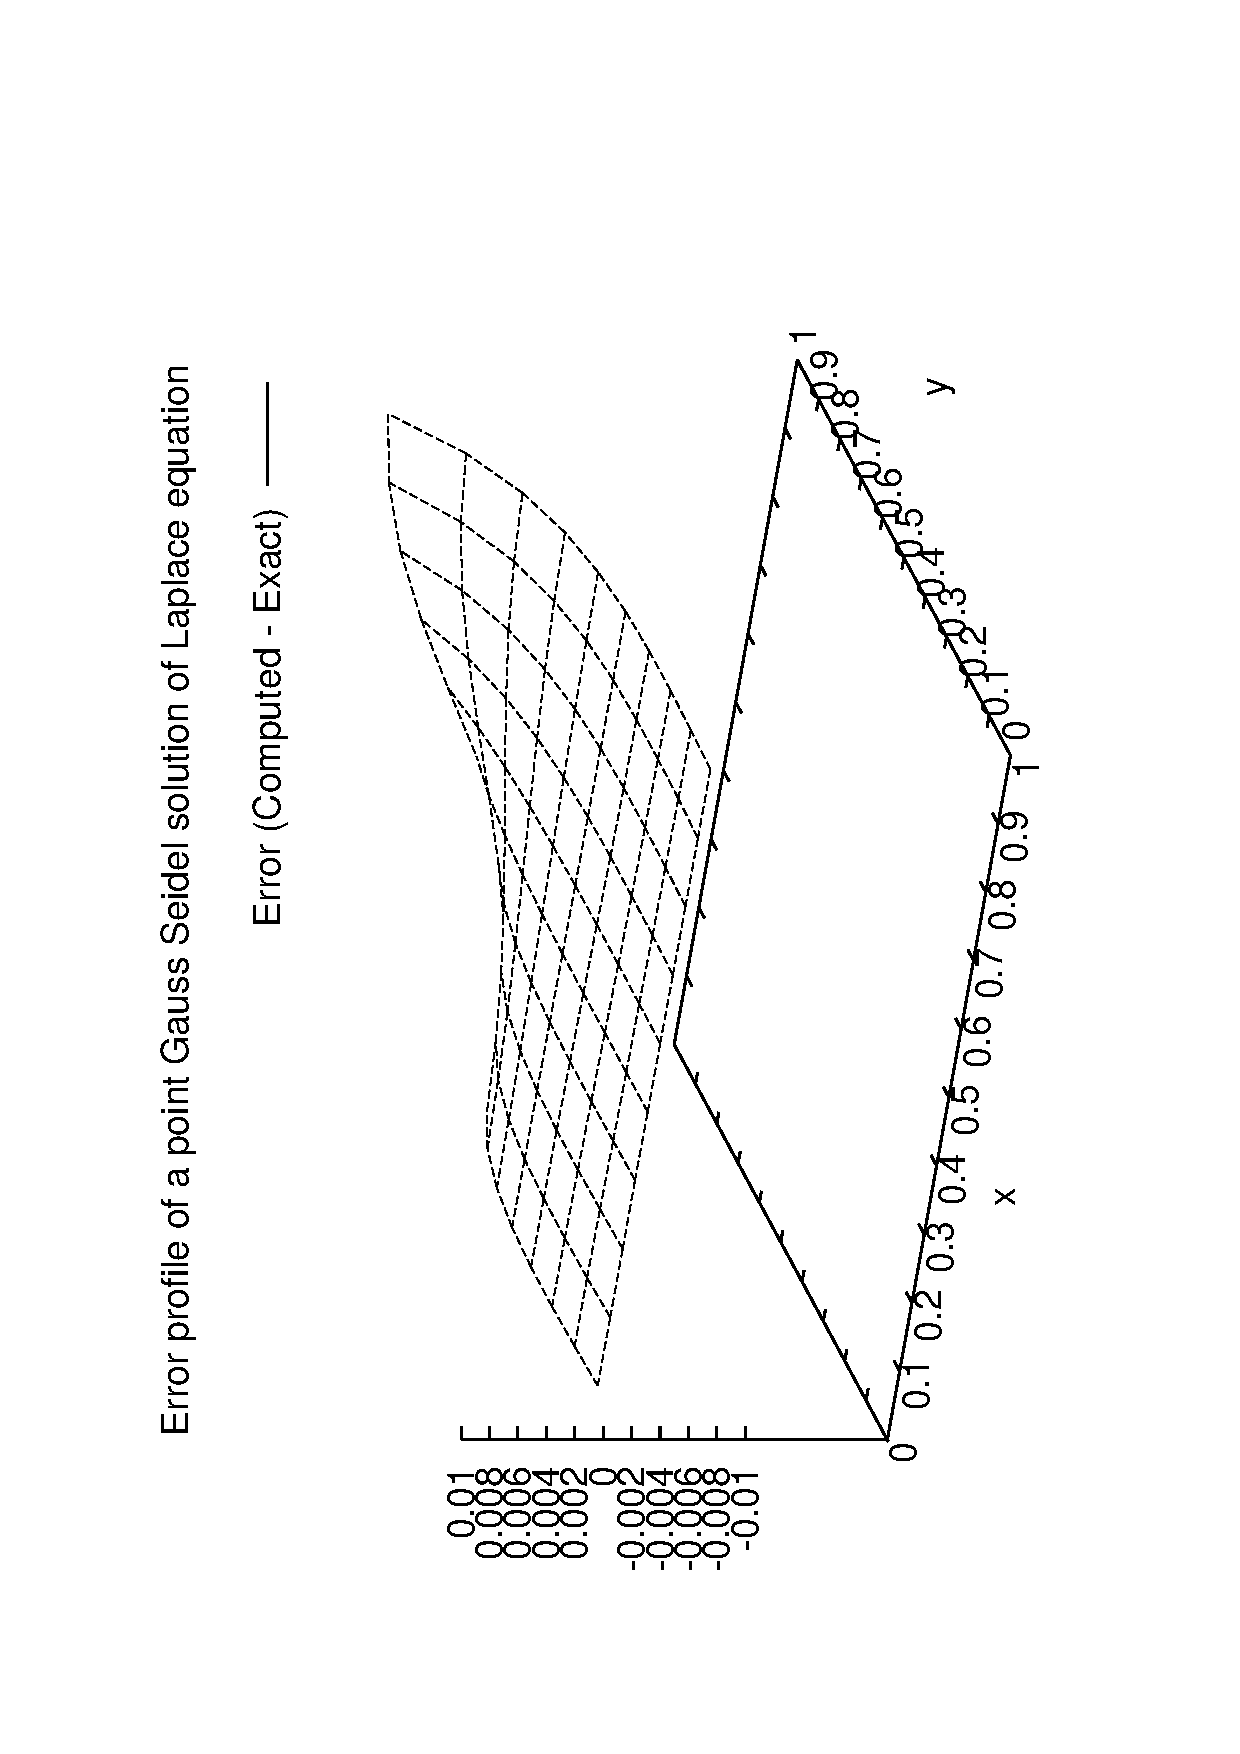
\includegraphics[width=0.5\textwidth, angle = -90]{../plots/mesh1/errors}
      \caption{Solution error in computing temperature distribution in a 10x10 computational domain. The solution exhibited less than $10^{-7}$ change per iteration after 205 iterations (without relaxation). The $L_2$ norm was calculated to be 0.00245704.}                
      \label{errors}
    \end{figure}
    
  \item Over-relaxation: After modifying the code to allow SOR, significant decreases in iteration counts were observed. With an over-relaxation coefficient ($\omega$ = 1.5), 87 iterations are taken to solve to an error norm of 0.00245703 given a maximum change of $10^{-7}$ per iteration. However, error norms stop changing only beginning with a maximum change of $10^{-8}$ per iteration. This constant error norm was found to be 0.00245704 (and was calculated over 120 iterations).
    
  \item Convergence behaviour: Three different relaxation parameters (1.0, 1.3, 1.5) were used to solve the Laplacian on the uniform grid. The maximum change in solution for every iteration has been plotted versus iterations in Figure~\ref{sor}.
    
    \begin{figure}
      \centering
      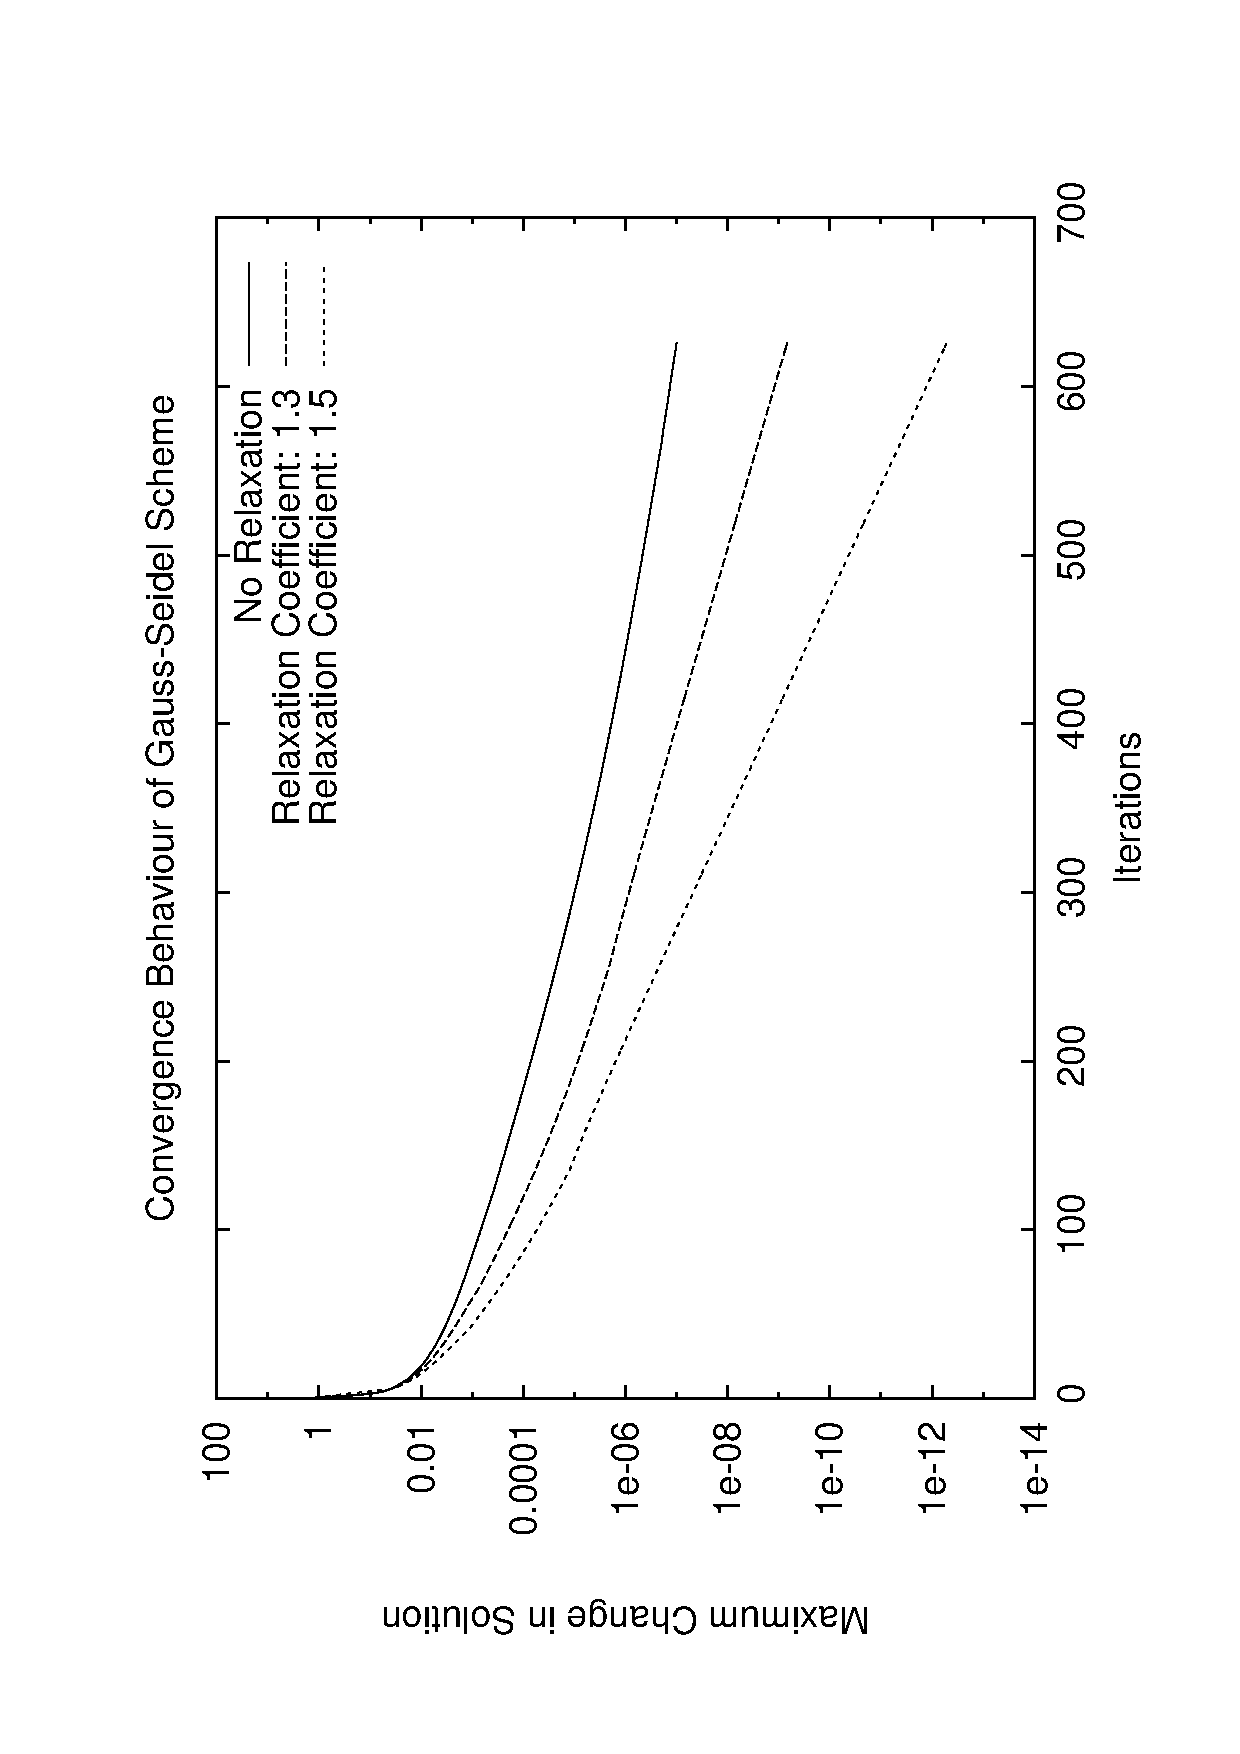
\includegraphics[width=0.5\textwidth, angle = -90]{../plots/mesh2/sor}
      \caption{Convergence behaviour of Gauss Seidel schemes on a 20x20 mesh. Iterations of 279, 400 and 626 were taken by over-relaxed (1.5, 1.3 and 1.0 respectively) solutions to converge. The over-relaxed iterations were allowed to proceed till the un-relaxed scheme converged.}          
      \label{sor}
    \end{figure}
    
  \item Accuracy: For order of accuracy estimation, 4 separate meshes (10x10, 20x20, 40x40, and 80x80) were used. The solution was made to converge in each mesh by making sure that error norm ($L_2$) does not change with iterations. This forces the limiting maximum change in solution per iteration to change for different sized meshes at the benefit of getting a better solution accuracy order (for e.g., with a fixed tolerance of $10^{-7}$, an order of 1.53 was observed, although with lesser iterations of 87, 279, 856, and 2508 respectively). The norm values follow a straight line (on a log graph) when plotted against local cell size of the structured mesh used. The slope of this line gives the observed order of method. Norm values have been tabulated in Table~\ref{table:norm} and plotted in Figure~\ref{norms}. The order of accuracy was found to be 1.985879 (verified using extrapolation technique).

    \begin{figure}
      \centering
      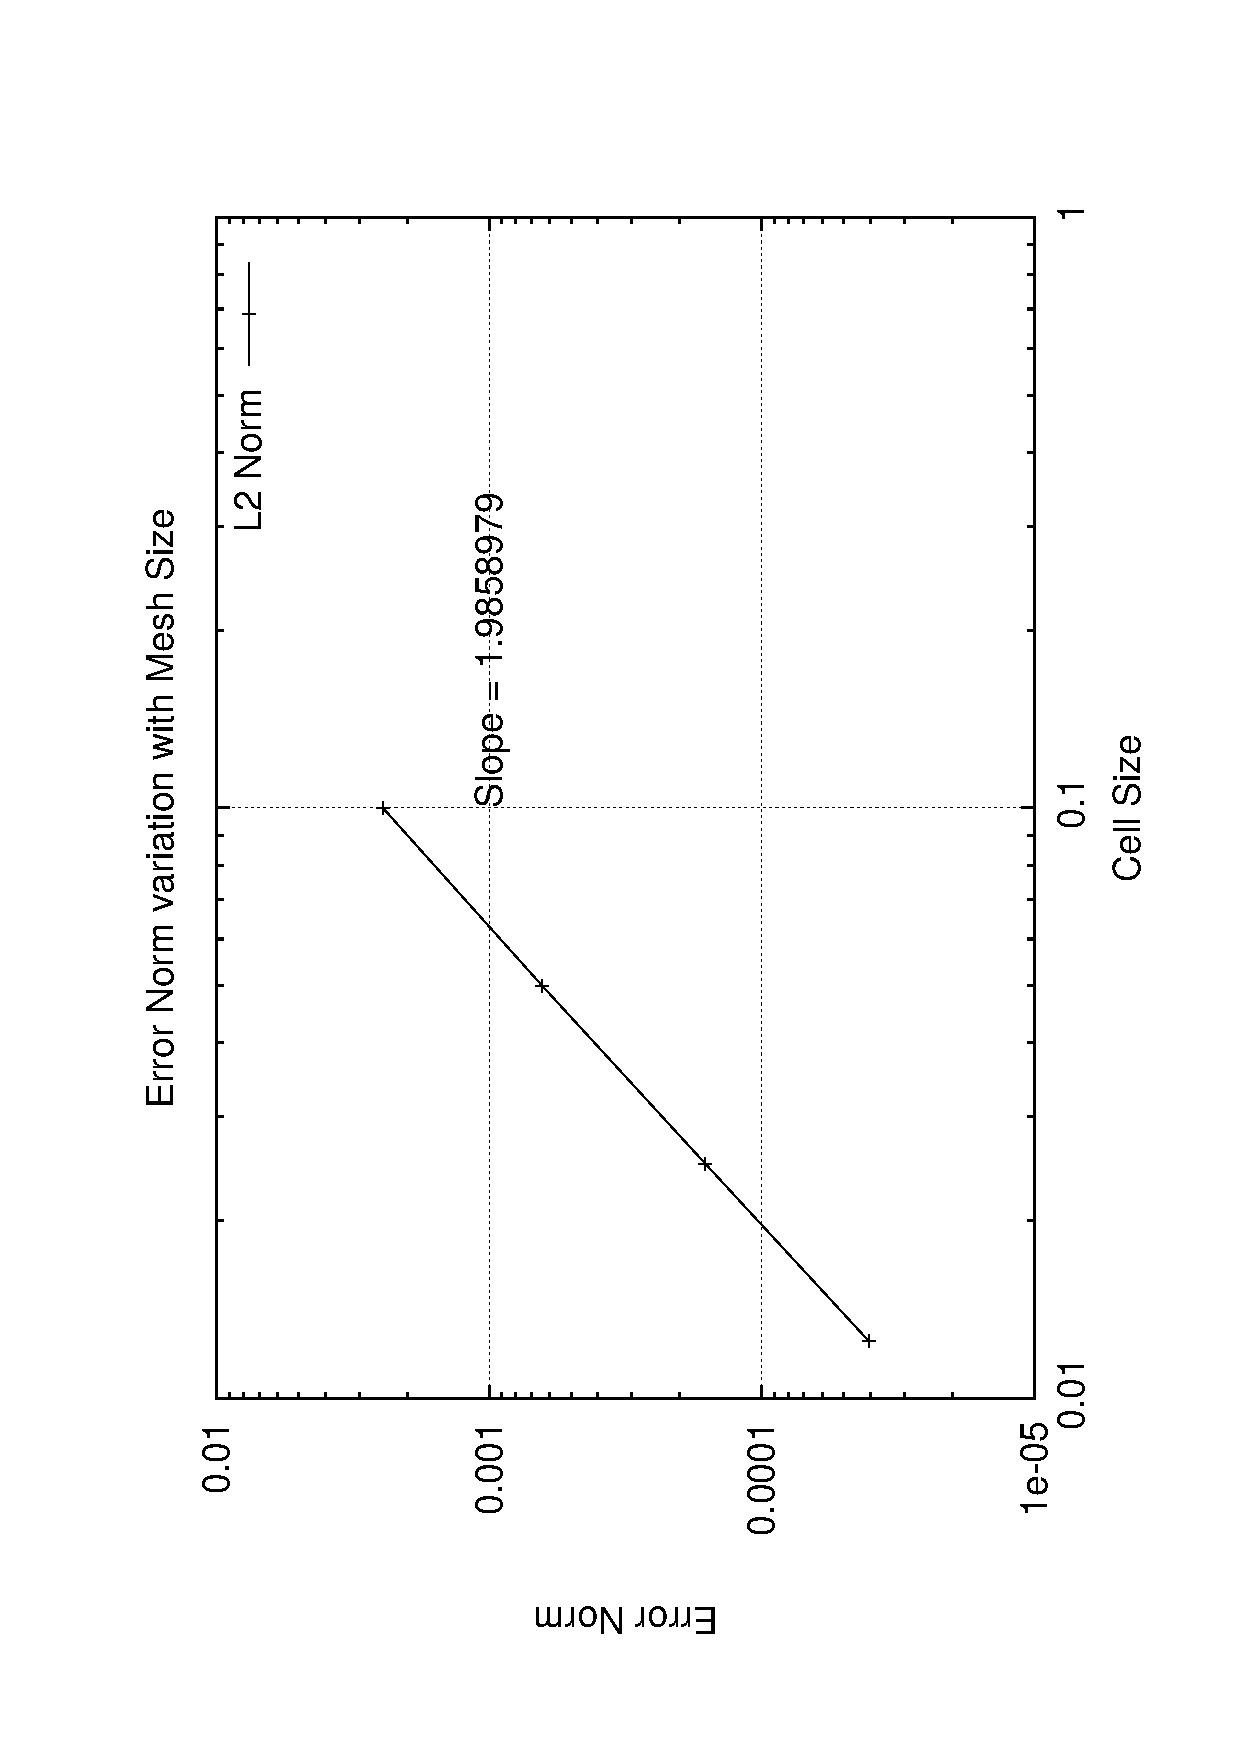
\includegraphics[width=0.5\textwidth, angle = -90]{../plots/mesh3/norm}
      \caption{Variation of $L_2$ norm with cell size shows a linear variation with the slope signifying the order of the method. Norms are larger for small mesh sizes because the finite volume averages tend to be significantly different from the local values for larger cell sizes.} 
      \label{norms}         
    \end{figure}
    
    \begin{table}
      \begin{center}
        \begin{tabular}{|l | c | c | r|}
          \hline
          Mesh Size & Convergence Criteria & Iterations & $L_2$ Norm\\
          \hline
          10x10 & $10^{-8}$ & 120 & 0.00245705 \\
          20x20 & $10^{-9}$ & 410 & 0.000638619\\
          40x40 & $10^{-10}$ & 1629 & 0.000161223\\
          80x80 & $10^{-11}$ & 6519 & 0.0000404044\\
          \hline
        \end{tabular}
        \caption{Convergence beahviour of solutions using point Gauss-Seidel iterative scheme with over-relaxation (1.5)}
        \label{table:norm}      
      \end{center}
    \end{table}
    
    \item Poisson problem in pressure calculation for incompressible flows: The following equation was solved in a uniform grid  spanning the domain 1x1 in dimensions.
    \begin{equation}
      \frac{\partial^2 P(x,y)}{\partial x^2} +   \frac{\partial^2 P(x,y)}{\partial y^2} = -{\left\{\frac{\partial u}{\partial x}\right\}}^2 +  2{\frac{\partial u}{\partial x}}{\frac{\partial v}{\partial y}} + {\left\{\frac{\partial v}{\partial y}\right\}}^2
    \end{equation}
    
    with the following velocity field and given boundary conditions.
    \begin{eqnarray}
      u = x^3 - 3xy^2\\
      v = -3x^2y + y^3
    \end{eqnarray}
    The source variation across the domain was simplified to the expression:
    
    \begin{equation}
      S = -18{(x^2 + y^2)}^2
    \end{equation}
    \begin{table}
      \begin{center}
        \begin{tabular}{|l | c | r|}
          \hline
          Mesh Size & Convergence Criteria & Iterations\\
          \hline
          20x20 & $10^{-8}$ & 1002\\
          40x40 & $10^{-8}$ & 2936\\
          80x80 & $10^{-8}$ & 12238\\
          \hline
        \end{tabular}
        \caption{Convergence behaviour of finite volume solutions of Poisson problem in pressure solved using point Gauss-Seidel scheme with over-relaxation 1.5}
        \label{table:norm2}      
      \end{center}
    \end{table}

    
    The ASME procedure for analysis of error and estimation of order was implemented for values of P($\frac{1}{2},\frac{1}{2}$) using 3 different meshes (20x20, 40x40 and 80x80) with constant grid refinement factor, r = 2 to simplify error estimation. With a maximum change per iteration of Gauss-Seidel taken as $10^{-7}$, the apparent order of the scheme was calculated as $\mathcal{O} \sim 1.75002$ and the solution was extrapolated to: $4.93743 \pm 2.35637 \times 10^{-5}$ taking iterations of 859, 2936, and 10173 respectively. The same scheme was run for a lower ($10^{-8}$) tolerance for the maximum solution change per solution, where the values obtained for P($\frac{1}{2},\frac{1}{2}$) stopped fluctuating. The apparent order for this scheme was improved to $\mathcal{O} \sim 1.972644$ and the extrapolated solution was $P = 4.9374927 \pm 1.633160 \times 10^{-5}$ i.e. a smaller error bound.

\end{itemize}

\emph{Comments:}
\begin{itemize}
\item Error profiles were found to match the actual temperature distribution. This is possible due to the fact that a 0 value specified boundary has little to go wrong, as compared to a cosine valued boundary. Errors in the calculation of the cosine, the value of pi, machine error etc show up in which case. For complicated grids (unstructured) the error is expected to numerically diffuse to a greater extent than this case.
  \item The iteration counts were reduced by sweeping the array starting from points in domain where neighbouring ghost cells contain maximum value (or atleast non-zero values). This way numerical diffusion is faster as compared to starting from 0 valued boundary condition. With small meshes this method works faster by a few iterations (4 in a mesh of 10x10 with no relaxation) and with larger meshes, significant savings are made (over 100 iterations in 80x80 mesh with 1.5 relaxation). However, it was noticed that since these converged (to a given maximum change per iteration) faster, the $L_2$ norms can be slightly larger ($\mathcal{O} \sim 10^{-7}$) than those obtained using a slower sweep pattern. This is perhaps due to the fact that given more time to diffuse, the solution converges to a value closer to the exact solution.
  \item Value of $\pi$ was used from Wikipedia. The constant M\_PI defined in math library seeps in errors and makes the iteration count for 10x10 mesh of Laplacian increase to 219 (without relaxation).
  \item The Gauss-Seidel scheme with relaxation was modified to include change in value ''after'' relaxation. Initially, the change was being measured before multiplying the relaxation coefficient to $\delta T_{i,j}$. Thus, a few iterations were compromised at the expense of increase in errors and hence, the change in code improved the order of the method.
  \item Convergence was established by finding the greatest tolerance below which the error norm was found to stay constant. This substantiates our choice for the cut-off point (of maximum solution change per iteration) used to declare convergence. This is of vital importance to the order (observed) of the numerical scheme. Different tolerances were required as the mesh size was increased. This shows that convergence becomes successively slower as the cell sizes are decreased, and as the solutions nears the convergence criteria (the given maximum change in solution per iteration).
  \item It is important to set a high precision of output numbers using \emph{setprecision(10)}. There was a fair improvement in the order of accuracy after including more digits.
\end{itemize}

\end{document}
